\subsection{Functional failure study}
\label{sec:failure-case-study}

% What is done here, what was the initial motivation
In this section, a practical case of functional failure of an integrated function is studied.
It was found on the integrated circuit described previously in \ref{sec:real-product-study}.
It was discovered while exploring the impact of reducing the amount of external devices on the robustness of the chip.
Reducing the amount of external devices is always interesting to lower the cost of an electronic system.

% How does it happen
The failure can be induced by injecting a negative-voltage \gls{esd} discharge on the battery input pin (Fig. \ref{XX}).
The \gls{ESD} is superimposed on the DC battery voltage, when the product is in operation.
This input is a realistic entry point for an \gls{esd}.
Indeed, it is connected directly to the integrated circuit, but it is exposed at the system level.
The battery is connected to this input by a cable, which is a frequent entry point for \gls{esd} (Source ?).

TODO: SCHEMA injection setup

% What is the result
The failure can be observed on the regulated 2.5V supplies, and in general on the entire system's behavior.
With a sufficiently large negative stress, the regulated output is disturbed and goes into soft-start (Fig. \ref{XX}).
A soft-start is a special sequence, normally happening when the device is first powered-on.
During this sequence, the supply voltage slowly rises from 0V to its nominal value, to avoid overshoots that could damage sensitive blocks.
Soft-starts can last from tens to hundreds of microseconds (source ?).
As a consequence the entire integrated functions are not available during the soft-start.
Some functions can be disturbed for much longer if they also need to follow their own startup sequences.

TODO: MEASUREMENT FAILURE OUTPUT

% Talk about the scale factor
To summarize, a negative stress of a hundred nanoseconds induces here a supply restart of tens of microseconds.
Parts of the system can be disturbed for much longer.
There is a scale factor of at least 100 between the stress width and the regulation function.
In this study, we try to explain how an \gls{esd} can generate such a scale factor.

\subsubsection{Study through simulation}

% Is the simulation accurate
To understand the failure mechanism, top-level simulations are first ran to see if the global failure can be reproduced.
A simulation setup is built to match closely the real circuit.
The \gls{tlp} model (described in section \ref{sec:tlp-modeling}) is also employed.
The external input and output voltage waveforms are compared in Fig. \ref{fig:wvf-vboost} (input) and Fig. \ref{fig:wvf-v2p5} (output).
Both curves correlate well, and the regulator restart is correctly reproduced in simulation.
These results tend to indicate that the simulations can be trusted for this study case.

% TODO: MEASUREMENT vs SIMULATION
\begin{figure}[!htbp]
  \centering
  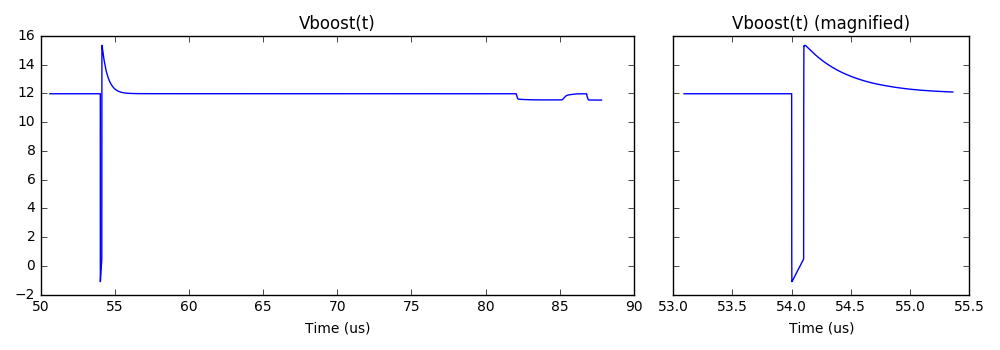
\includegraphics[width=0.9\textwidth]{src/3/figures/vboost.png}
  \caption{Waveform of the vboost input pin}
  \label{fig:wvf-vboost}
\end{figure}

\begin{figure}[!htbp]
  \centering
  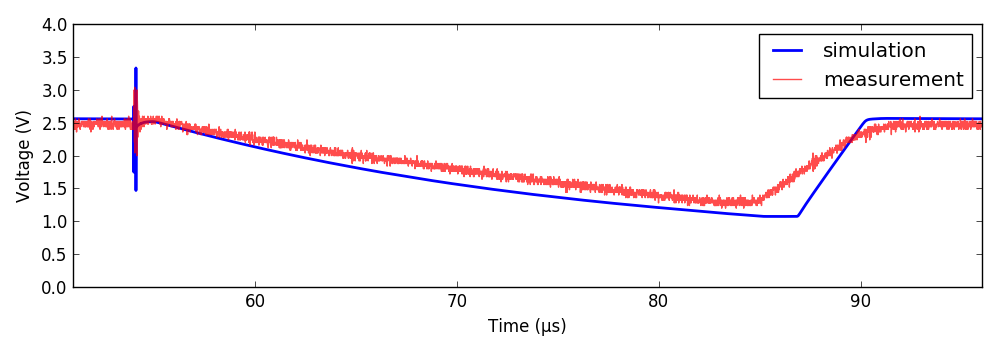
\includegraphics[width=0.9\textwidth]{src/3/figures/v2p5.png}
  \caption{Waveform of the v2p5 output pin}
  \label{fig:wvf-v2p5}
\end{figure}

% Make the investigation
The investigation process is now conducted.
The injected stress is a rectangular pulse of -100V amplitude and 100ns width.
The main output of the first block (the pre-regulator) is observed in simulation (Fig. \ref{fig:wvf-vclamp9}).
At 54 \textmugreek{}s, its \textit{vclamp9} output voltage is clearly disturbed by the negative stress.
The net reaches as low as 0V for a brief amount of time.
Overall, the net is disturbed for 750 ns.

% Next net, bandgap input
In turn, this net powers the bandgap reference.
Thus, it can be expected that the bandgap is going to be disturbed as well.
The observation of the 1.0V bandgap reference \textit{vref1p0} confirms it (Fig. \ref{fig:wvf-v1p0}).
The reference drops down to 0.25V, and is disturbed for about 3 \textmugreek{}s.

\begin{figure}[!htbp]
  \centering
  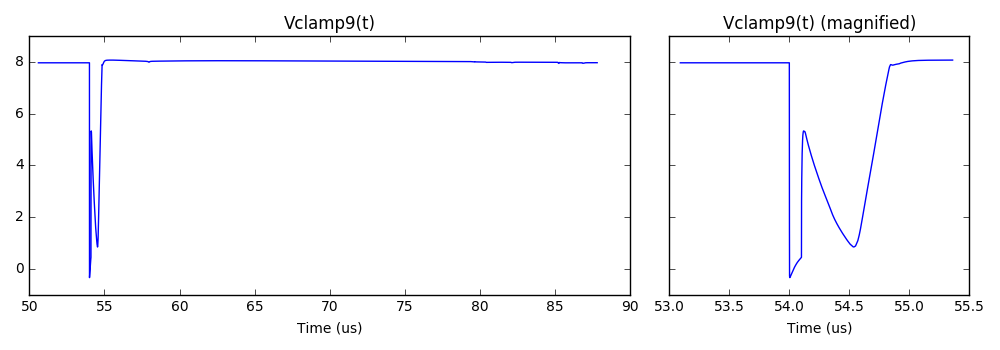
\includegraphics[width=0.9\textwidth]{src/3/figures/vclamp9.png}
  \caption{Waveform of the vclamp9 internal net}
  \label{fig:wvf-vclamp9}
\end{figure}

\begin{figure}[!htbp]
  \centering
  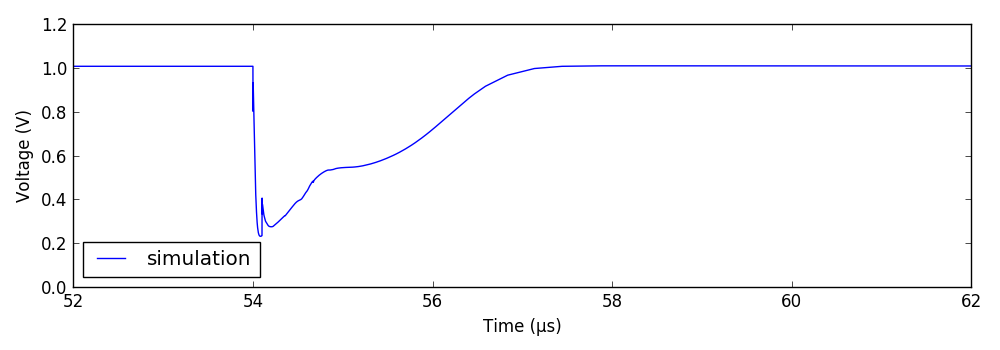
\includegraphics[width=0.9\textwidth]{src/3/figures/v1p0.png}
  \caption{Waveform of the vref1p0 internal net}
  \label{fig:wvf-v1p0}
\end{figure}

% Final net
Finally, this bandgap reference is used by the regulator to generate the 2.5 V external supply output.
Net \textit{v2p5} drops below 1.5V, and is disturbed for more than 30 \textmugreek{}s.
Clearly, the scale factor is well reproduced in the simulation.

% Preliminary conclusion with scale factor
In the first block (pre-regulator), the disturbance width increased from 100 ns to 750 ns.
In the second block (bandgap), it increased from 750 ns to 3 \textmugreek{}s.
In the third block (regulator), it reached 30 \textmugreek{}s.
In each block, there is an aggravation of the failure.

% Talk about failure in cascade
%TODO: Review next
It appears there is a failure in cascade of the regulation function.
When the disturbance propagates through a block, it is amplified and becomes more severe.
Time is a key parameter here.
If the disturbance only affected the final output for 100 ns, the integrated circuit functionnality would most likely not be affected.
WHY ?
%TODO: Detail more. Duration key parameter here

% What is really causing the failure
%TODO: Detail
Soft-start, what can impact it ?
WHICH SIGNAL IS GOING out of spec first ?

%TODO; Talk about hypothesis that this is why system is failing, but maybe it is more complex than that.
So far rely exclusively on simulations.
To confirm the simulation, and acquire more internal data, a testchip is designed.
